In the following experiment the effects of ego depletion on social risk with regard to con-sumer behaviour and behaviour in general will be examined. In order to analyse social risk and consumer behaviour the experiment aims for a decision between products with supposedly high versus low social risk. The second part of the questionnaire includes a scenario in which participants were confronted with criminal cases (judges’ dilemma). This test was included in order to check if ego depletion has an effect on social risk related decision-making in different contexts as well and not only in the context of purchase decisions, thus possibly supporting our results. Participants were provided with information of the respective perpetrator’s criminal record\footnote{All judges’ cases are fictitious} and his/her behaviour in custody. The awareness of responsibility regarding the decision if a ‘delinquent remains in custody’ or ‘will be granted probation’ involves the concept of social risk.
The main components of the empirical research are divided into three subcategories. 
\begin{enumerate}
\item The depletion task (Stroop test)
\item The self-evaluation 
\item The decision-making task (products/judges’ dilemma)
\end{enumerate}
Before the structure of the survey will be discussed in detail, the two parts of the question-naire have to be examined. Under the assumption that social risk is a significant factor in the decision-making process, two pre-tests of the survey were implemented. Both parts aim at the aspect of decision-making and social risk. The first and main part focuses on the decision-making process (as part of a purchase decision) under ego depletion, whereas the second part observes the decision-making process in judicial decisions under ego depletion. 
\section{Pre-Test}
The pre-tests were designed in order to define the framework of ‘social risk’. Therefore, we conducted one survey, which dealt with the question of social risk regarding consumer decisions. The other one observed the term of social risk in regard to judicial cases. Both pre-tests will be more closely examined in the two following subsections.
\subsection{Consumer Choice}
The sample consisted of 34 students (21 male / 13 female) aged between 19 and 32 (m = 25,41; SD = 4,28) enrolled at the University of Hamburg. The main dependent measure for the pre-test was social risk on consumer choice. Participants were presented with a set of products. Each product could be distinguished by one attribute, either colour or design. Partici-pants were randomly assigned to two groups and were shown sets of either five or six products, depending on the group. Each product was presented in five different colours or designs. \par
In the first step, participants were instructed to rank all five versions of the same prod-uct according to social risk. The following definition of social risk was given: (a) the colour or design of which they would most likely expect positive reactions of their social environment (low risk) versus (b) the product of which they would most likely expect adverse reactions of their social environment (high risk). In the second step, participants had to rank all five ver-sions according to personal preference (in the following referred to as ‘liking scale’). The last step aimed for a consumer decision. Participants had to rank the product itself with the help of a Likert scale, with the variables being (a) social risk and (b) design as significant for a purchase decision. A sample of the questionnaire is pictured in figure \ref{fig:pretest_sample_shoes}. To emphasize the scale visually in the questionnaire a grey shadowed triangle was put behind the scale.\par
\begin{figure}[h!]
\center
	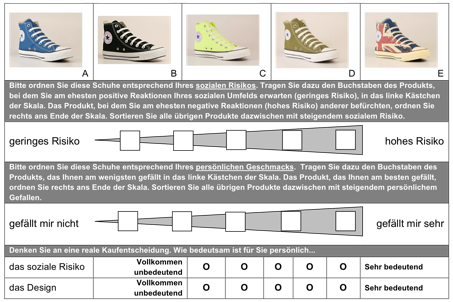
\includegraphics[width=1\textwidth]{images/pretest_sample_shoes.png}
  \caption{Sample of questions raised in the pre-test (products) are displayed. The upper task requests to estimate the ‘social risk’ of the product. The following task requests to estimate the ‘liking’ of the product. The lower task re-quests to estimate the personal importance of ‘social risk’ and ‘design’ in a purchase decision.}\label{fig:pretest_sample_shoes}
\end{figure}
Products were chosen to be part of the final questionnaire based on the premise that they pro-vided an approximately equivalent liking and a preferably diverse social risk. Four of the elev-en products complied with our expectations (shoes, sofa, wine, mp3 player and car). \par
Figure \ref{fig:pretest_shoes} displays the five alternatives regarding the product ‘shoes’. The variation ‘black’ with a low ‘social risk’ rating and the variation ‘yellow’ with a high ‘social risk’ rating would indicate the maximum of difference between the variable ‘social risk’. The ‘liking’ rate of these two product variations, however, show also the highest deviation. Therefore, we de-cided to select the product ‘shoe’ with the attribute ‘blue’ (SR = 2.06; liking = 3.50) as the low social risk, and the ‘union jack’ (SR =  4.12; liking = 2.87) as the high social risk alterna-tive. In addition the product choices regarding the variable ‘liking’ corresponded more strongly with each other. 
% \begin{figure}[h!]
% \center
% 	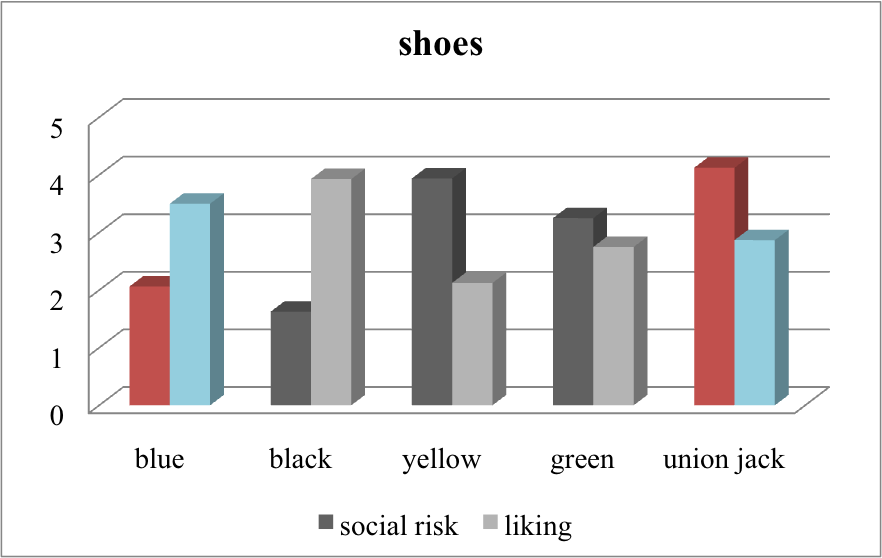
\includegraphics[width=0.9\textwidth]{images/pretest_shoes.png}
%   \caption{The results of the pre-test with regard to the product ‘shoes’ are displayed. The chosen products for the final survey are highlighted in colour (‘social risk’= red and ‘liking’ = blue). The ordinate denotes ‘social risk’ and ‘liking’ on a scale ranging from zero to five. The abscissa denotes the product in five different ‘colour’ variants.}\label{fig:pretest_shoes}
% \end{figure}
Figure \ref{fig:pretest_mp3} displays the options for the product ‘mp3 player’. In this case we decided to select the product ‘mp3 player’ with the attribute ‘yellow’ (SR = 3.88; liking = 2.71) which corresponds more strongly with alternative ‘red’ in regard to the ‘liking’ (SR =  3.29; liking = 2.59). Although, the disparity of social risk would have been higher with the ‘purple’ mp3 player, we decided that the equality of the ‘liking’ as a comparable foundation appears to be more important than finding the highest possible difference in value regarding the item social risk.
% \begin{figure}[h!]
% \center
% 	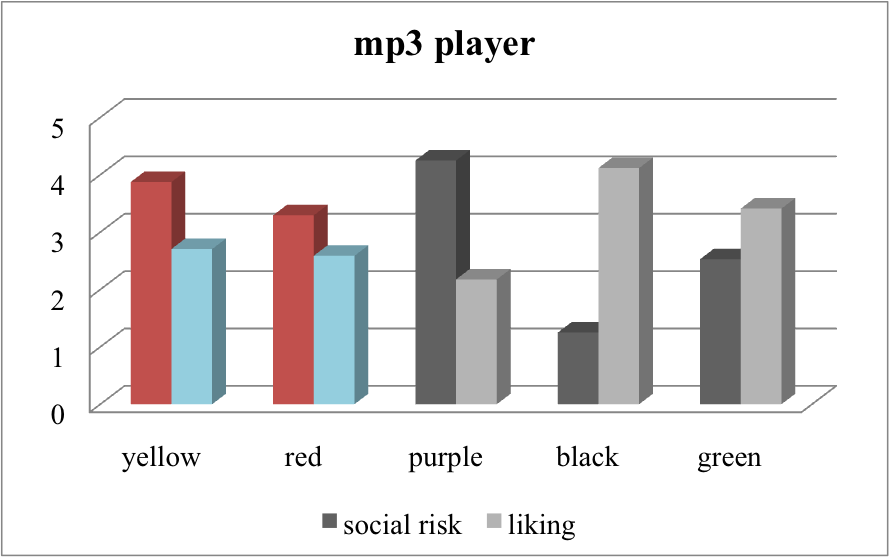
\includegraphics[width=0.9\textwidth]{images/pretest_mp3.png}
%   \caption{The results of the pre-test with regard to the product ‘mp3 player’ are displayed. The chosen products for the final survey are highlighted in colour (‘social risk’= red and ‘liking’ = blue). The ordinate denotes ‘social risk’ and ‘liking’ on a scale ranging from zero to five. The abscissa denotes the product in five different ‘colour’ variants.}\label{fig:pretest_mp3}
% \end{figure}
Figure \ref{fig:pretest_sofa} displays the options for the product ‘sofa’. In this case we decided to select the product ‘sofa’ with the attribute ‘red’ (SR = 3.88; liking = 3.19) which corresponds more strongly with alternative ‘grey’ in regard to the ‘liking’ (SR = 2.69; liking = 3,25). Again, we decided that the equality of the ‘liking’ as a comparable foundation appears to be more im-portant than finding the highest possible difference in value regarding the item social risk. 
% \begin{figure}[h!]
% \center
% 	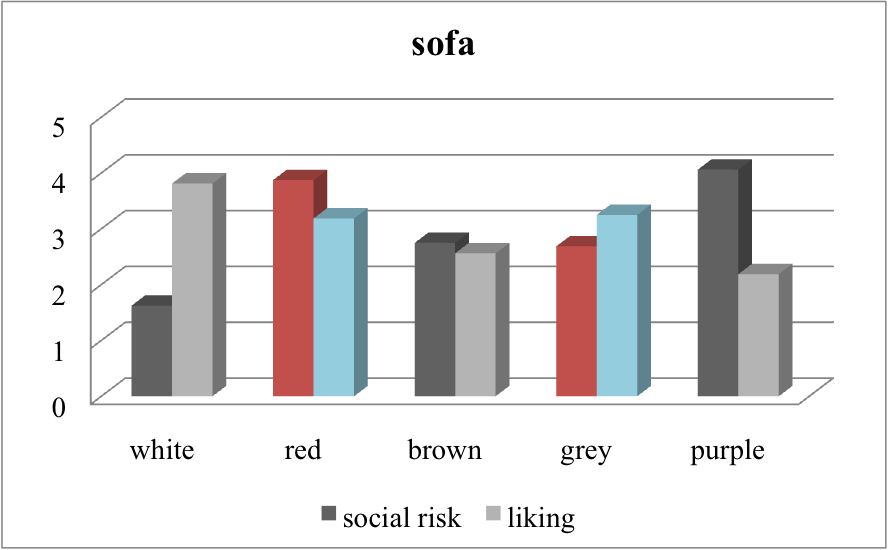
\includegraphics[width=0.9\textwidth]{images/pretest_sofa.png}
%   \caption{The results of the pre-test with regard to the product ‘sofa’ are displayed. The chosen products for the final survey are highlighted in colour (‘social risk’= red and ‘liking’ = blue). The ordinate denotes ‘social risk’ and ‘liking’ on a scale ranging from zero to five. The abscissa denotes the product in five different ‘colour’ variants.}\label{fig:pretest_sofa}
% \end{figure}
Figure \ref{fig:pretest_cars} displays the five alternatives regarding the product ‘car’. This time the distinctive attribute is ‘design’ not ‘colour’. For this purpose we chose five different cars from the same manufacturer and in the same colour. Therefore, we decided to select the product ‘car’ with the attribute ‘limousine’ (SR = 2.12; liking = 2.94) as the low social risk, and the ‘SUV’ (SR =  3.41; liking = 3.29) as the high social risk alternative. In addition the product choices regard-ing the variable ‘liking’ corresponded more strongly with each other than the other possible combinations.
% \begin{figure}[h!]
% \center
% 	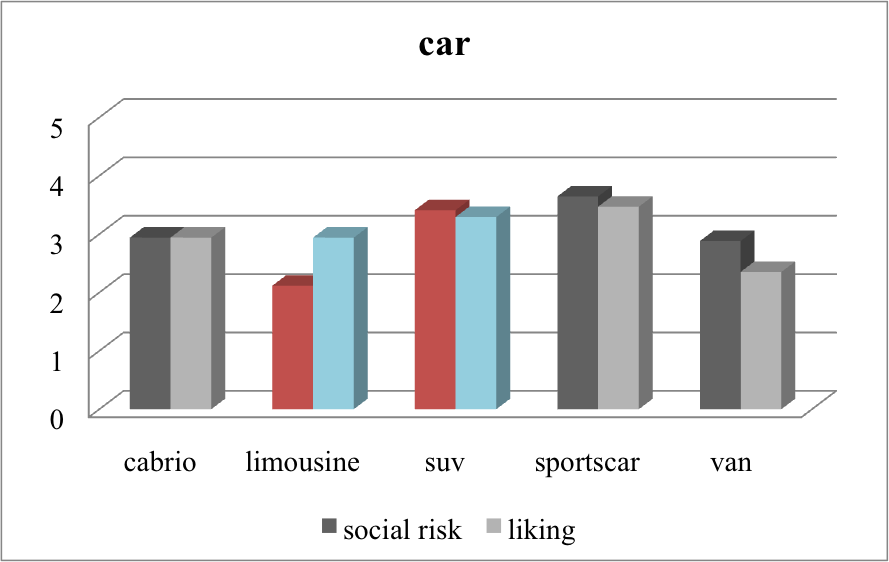
\includegraphics[width=0.9\textwidth]{images/pretest_cars.png}
%   \caption{The results of the pre-test with regard to the product ‘cars’ are displayed. The chosen products for the final survey are highlighted in colour (‘social risk’= red and ‘liking’ = blue). The ordinate denotes ‘social risk’ and ‘liking’ on a scale ranging from zero to five. The abscissa denotes the product in five different ‘design’ variants.}\label{fig:pretest_cars}
% \end{figure}
Figure \ref{fig:pretest_wine} displays the options for the product ‘wine label’. In this case we decided to select the product ‘wine label’ with the attribute ‘white/green’ (SR = 3.36; liking = 3.07) as the high ‘social risk’ item, which also corresponds with the strongest alternative and low ‘social risk’ item ‘green/gold’ regarding the ‘liking’ (SR =  2.50; liking = 3.21). 
% \begin{figure}[h!]
% \center
% 	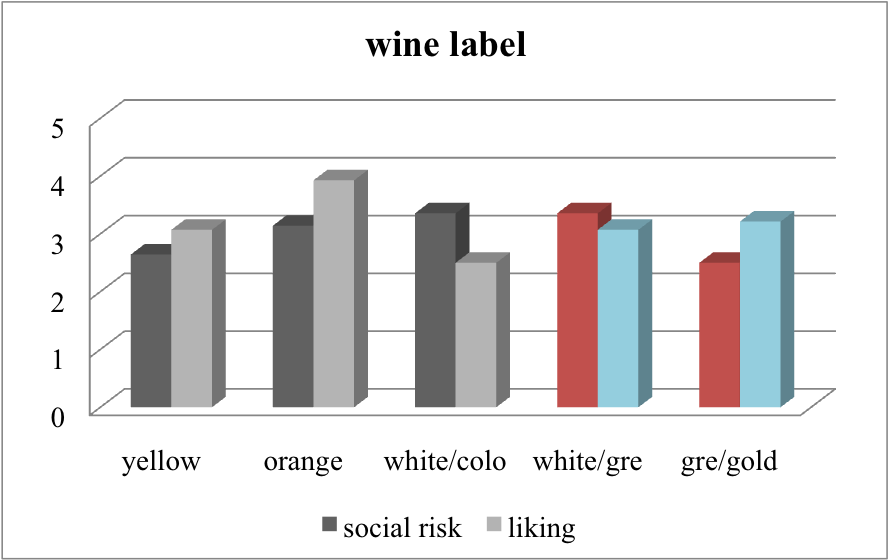
\includegraphics[width=0.9\textwidth]{images/pretest_wine.png}
%   \caption{The results of the pre-test with regard to the product ‘wine label’ are displayed. The chosen products for the final survey are highlighted in colour (‘social risk’= red and ‘liking’ = blue). The ordinate denotes ‘social risk’ and ‘liking’ on a scale ranging from zero to five. The abscissa denotes the product in five different ‘colour’ variants.}\label{fig:pretest_wine}
% \end{figure}

\begin{figure}[h!]
  \begin{center}
    % \showthe\columnwidth % Use this to determine the width of the figure.
    \subfloat[]{\label{fig:pretest_shoes}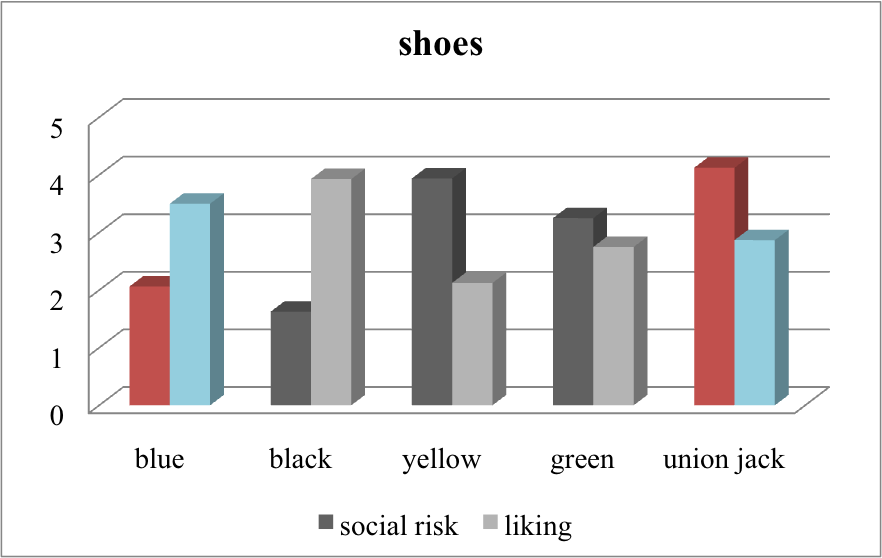
\includegraphics[width=220pt]{images/pretest_shoes.png}}\hspace{1pt}
    \subfloat[]{\label{fig:pretest_mp3}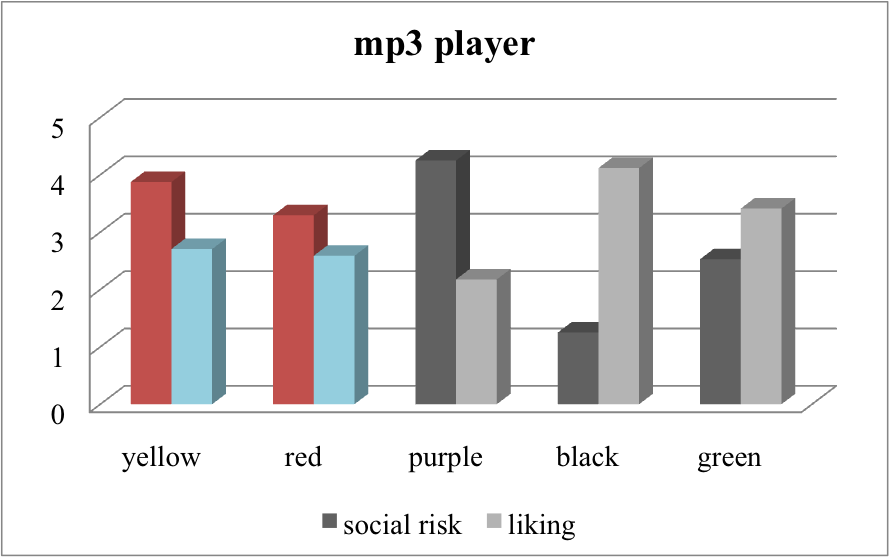
\includegraphics[width=220pt]{images/pretest_mp3}}\\
    \caption{The results of the pre-test with regard to the product ‘wine label’ are displayed. The chosen products for the final survey are highlighted in colour (‘social risk’= red and ‘liking’ = blue). The ordinate denotes ‘social risk’ and ‘liking’ on a scale ranging from zero to five. The abscissa denotes the product in five different ‘colour’ variants.}\label{fig:pretests}
  \end{center}
\end{figure}